% Options for packages loaded elsewhere
\PassOptionsToPackage{unicode}{hyperref}
\PassOptionsToPackage{hyphens}{url}
%
\documentclass[
  11pt,
]{article}
\usepackage{amsmath,amssymb}
\usepackage{lmodern}
\usepackage{ifxetex,ifluatex}
\ifnum 0\ifxetex 1\fi\ifluatex 1\fi=0 % if pdftex
  \usepackage[T1]{fontenc}
  \usepackage[utf8]{inputenc}
  \usepackage{textcomp} % provide euro and other symbols
\else % if luatex or xetex
  \usepackage{unicode-math}
  \defaultfontfeatures{Scale=MatchLowercase}
  \defaultfontfeatures[\rmfamily]{Ligatures=TeX,Scale=1}
\fi
% Use upquote if available, for straight quotes in verbatim environments
\IfFileExists{upquote.sty}{\usepackage{upquote}}{}
\IfFileExists{microtype.sty}{% use microtype if available
  \usepackage[]{microtype}
  \UseMicrotypeSet[protrusion]{basicmath} % disable protrusion for tt fonts
}{}
\makeatletter
\@ifundefined{KOMAClassName}{% if non-KOMA class
  \IfFileExists{parskip.sty}{%
    \usepackage{parskip}
  }{% else
    \setlength{\parindent}{0pt}
    \setlength{\parskip}{6pt plus 2pt minus 1pt}}
}{% if KOMA class
  \KOMAoptions{parskip=half}}
\makeatother
\usepackage{xcolor}
\IfFileExists{xurl.sty}{\usepackage{xurl}}{} % add URL line breaks if available
\IfFileExists{bookmark.sty}{\usepackage{bookmark}}{\usepackage{hyperref}}
\hypersetup{
  pdftitle={10. Assessment of the Northern Rockfish stock in the Gulf of Alaska},
  pdfauthor={Benjamin C. Williams, Peter-John F. Hulson, Chris R. Lunsford},
  hidelinks,
  pdfcreator={LaTeX via pandoc}}
\urlstyle{same} % disable monospaced font for URLs
\usepackage[top=1in,bottom=1in,left=1in,right=1in]{geometry}
\usepackage{longtable,booktabs,array}
\usepackage{calc} % for calculating minipage widths
% Correct order of tables after \paragraph or \subparagraph
\usepackage{etoolbox}
\makeatletter
\patchcmd\longtable{\par}{\if@noskipsec\mbox{}\fi\par}{}{}
\makeatother
% Allow footnotes in longtable head/foot
\IfFileExists{footnotehyper.sty}{\usepackage{footnotehyper}}{\usepackage{footnote}}
\makesavenoteenv{longtable}
\usepackage{graphicx}
\makeatletter
\def\maxwidth{\ifdim\Gin@nat@width>\linewidth\linewidth\else\Gin@nat@width\fi}
\def\maxheight{\ifdim\Gin@nat@height>\textheight\textheight\else\Gin@nat@height\fi}
\makeatother
% Scale images if necessary, so that they will not overflow the page
% margins by default, and it is still possible to overwrite the defaults
% using explicit options in \includegraphics[width, height, ...]{}
\setkeys{Gin}{width=\maxwidth,height=\maxheight,keepaspectratio}
% Set default figure placement to htbp
\makeatletter
\def\fps@figure{htbp}
\makeatother
\setlength{\emergencystretch}{3em} % prevent overfull lines
\providecommand{\tightlist}{%
  \setlength{\itemsep}{0pt}\setlength{\parskip}{0pt}}
\setcounter{secnumdepth}{-\maxdimen} % remove section numbering
\usepackage{multirow} \usepackage{float} \usepackage{booktabs} \usepackage{colortbl} \usepackage{graphicx} \usepackage{sectsty} \usepackage{babel} \allsectionsfont{\centering} \usepackage{array} \newcolumntype{R}{>{\centering\arraybackslash}m{1.9cm}} \newcolumntype{L}[1]{>{\raggedright\let\newline\\\arraybackslash\hspace{0pt}}m{#1}} \makeatletter \renewcommand{\figurename}{Figure 10-\@gobble} \makeatother \makeatletter \renewcommand{\tablename}{Table 10-\@gobble} \makeatother \usepackage{titlesec} \titlespacing\section{-5pt}{12pt plus 4pt minus 2pt}{0pt plus 2pt minus 2pt}
\ifluatex
  \usepackage{selnolig}  % disable illegal ligatures
\fi
\newlength{\cslhangindent}
\setlength{\cslhangindent}{1.5em}
\newlength{\csllabelwidth}
\setlength{\csllabelwidth}{3em}
\newenvironment{CSLReferences}[2] % #1 hanging-ident, #2 entry spacing
 {% don't indent paragraphs
  \setlength{\parindent}{0pt}
  % turn on hanging indent if param 1 is 1
  \ifodd #1 \everypar{\setlength{\hangindent}{\cslhangindent}}\ignorespaces\fi
  % set entry spacing
  \ifnum #2 > 0
  \setlength{\parskip}{#2\baselineskip}
  \fi
 }%
 {}
\usepackage{calc}
\newcommand{\CSLBlock}[1]{#1\hfill\break}
\newcommand{\CSLLeftMargin}[1]{\parbox[t]{\csllabelwidth}{#1}}
\newcommand{\CSLRightInline}[1]{\parbox[t]{\linewidth - \csllabelwidth}{#1}\break}
\newcommand{\CSLIndent}[1]{\hspace{\cslhangindent}#1}

\title{10. Assessment of the Northern Rockfish stock in the Gulf of Alaska}
\author{Benjamin C. Williams, Peter-John F. Hulson, Chris R. Lunsford}
\date{November 2021}

\begin{document}
\maketitle

\pagenumbering{gobble}

\hypertarget{executive-summary}{%
\section{Executive summary}\label{executive-summary}}

We use a statistical age-structured model as the primary assessment tool for GOA northern rockfish (\emph{Sebastes ciliatus}) which qualifies as a Tier 3 stock.
This assessment consists of a population model, which uses survey and fishery data to generate a historical time series of population estimates, and a projection model, which uses results from the population model to predict future population estimates and recommended harvest levels.
The data used in this assessment includes total catch biomass, fishery age and size compositions, trawl survey abundance estimates, and trawl survey age compositions.
For a partial assessment, we do not re-run the assessment model, but do update the projection model with new catch information.
This incorporates the most current catch information without re-estimating model parameters and biological reference points.
Full assessments for northern rockfish are conducted in even years and partial assessments in odd years.
For Gulf of Alaska northern rockfish in 2021, we present a partial assessment with updated projection model results to recommend harvest levels for the next two years.

\allsectionsfont{\raggedright}

\hypertarget{summary-of-changes-in-assessment-inputs}{%
\subsection{Summary of Changes in Assessment Inputs}\label{summary-of-changes-in-assessment-inputs}}

\emph{Changes in the input data:} There were no changes made to the assessment model inputs as this is an off-cycle year.
New data added to the projection model included updated catch data from 2020 (2,385 t) and new estimated catches for 2021-2023.
Catch data were queried on 2021-10-22, with the most recent catches in the query on 2021-10-16.
The 2021 catch was estimated by increasing the official catch as of 2021-10-16 by an expansion factor of 1.045, which accounts for the average fraction of catch taken after October 16 in the last three complete years (2018-2020).
This expansion factor results in an estimated catch for 2021 of 2,471 t.
To estimate future catches, we updated the yield ratio to 0.6, which was the average ratio of catch to ABC for the last three complete catch years (2018-2020).
This yield ratio was multiplied by the projected ABCs from the updated projection model to generate catches of 3,089 t in 2022 and 2,884 t in 2023.

\emph{Changes in assessment methodology:} There were no changes from the 2020 assessment (Williams \emph{et al.} 2020) since this is an off-cycle year.

\allsectionsfont{\raggedright}

\hypertarget{summary-of-results}{%
\subsection{Summary of Results}\label{summary-of-results}}

\emph{ABC recommendation}\\
For the 2022 fishery, we recommend maximum allowable ABC of 5,147 t from the updated projection model.
This ABC is a minor increase than the 2022 projected ABC of 5,100 t from the 2020 full assessment.

The stock is not being subject to overfishing, is not currently overfished, nor is it approaching a condition of being overfished.
The test for determining whether overfishing is occurring is based on the 2020 catch compared to OFL.
The official total catch for 2020 is 2,385 t which is less than the 2020 OFL of 6,396 t; therefore, the stock is not being subjected to overfishing.
The tests for evaluating whether a stock is overfished or approaching a condition of being overfished require examining model projections of spawning biomass relative to \(B_{35\%}\) for 2022 and 2023.
The estimates of spawning biomass for 2022 and 2023 from the current year projection model are 40,474 t and 37,408 t, respectively.
Both estimates are above the \(B_{35\%}\) estimate of 29,691 t and, therefore, the stock is not currently overfished nor approaching an overfished condition.

Reference values for northern rockfish are summarized in the following table, with the recommended ABC and OFL values in bold.

\begin{center}
\begin{tabular}{ |lcccc|}
\hline
 & \multicolumn{2}{c}{\cellcolor[gray]{0.9} As estimated or} & 
    \multicolumn{2}{c|}{As estimated or}\\
 & \multicolumn{2}{c}{\cellcolor[gray]{0.9} specified \emph{last} year for:} & 
    \multicolumn{2}{c|}{specified \emph{this} year for:}\\
    
 \textbf{Quantity/Status}                 & \cellcolor[gray]{0.9} 2021    & \cellcolor[gray]{0.9} 2022   & 2022* & 2023*\\ 
 \hline
    M (natural mortality)                 & \cellcolor[gray]{0.9} 0.07    &\cellcolor[gray]{0.9} 0.07    &  0.07  & 0.07\\
    Tier                                  & \cellcolor[gray]{0.9} 3a      & \cellcolor[gray]{0.9} 3a     & 3a & 3a\\
    Projected total (age 2+) biomass (t)  & \cellcolor[gray]{0.9} 102,715 & \cellcolor[gray]{0.9} 99,957 & 100,371 &    96,045 \\
    Projected female spawning biomass (t) & \cellcolor[gray]{0.9} 42,791  & \cellcolor[gray]{0.9} 40,462 & 40,474 & 37,408 \\
    $B_{100\%}$                           & \cellcolor[gray]{0.9} 84,832  & \cellcolor[gray]{0.9} 84,832 & 84,832   & 84,832 \\
    $B_{40\%}$                            & \cellcolor[gray]{0.9} 33,933  & \cellcolor[gray]{0.9} 33,933 & 33,933 & 33,933 \\
    $B_{35\%}$                            & \cellcolor[gray]{0.9} 29,691  & \cellcolor[gray]{0.9} 29,691 & 29,691    & 29,691 \\
  $F_{OFL}$                               & \cellcolor[gray]{0.9} 0.073   & \cellcolor[gray]{0.9} 0.073  & 0.073 & 0.073\\
   $maxF_{ABC}$                           & \cellcolor[gray]{0.9} 0.061   & \cellcolor[gray]{0.9} 0.061  & 0.061 & 0.061\\
   $F_{ABC}$                              & \cellcolor[gray]{0.9} 0.061   & \cellcolor[gray]{0.9} 0.061  & 0.061 & 0.061\\
    OFL                                   & \cellcolor[gray]{0.9} 6,396   & \cellcolor[gray]{0.9} 6,088  & \bf{6,143} & 5,874 \\
    maxABC (t)                            & \cellcolor[gray]{0.9} 5,358   & \cellcolor[gray]{0.9} 5,100  & \bf{5,147} & 4,921 \\
     ABC (t)                              & \cellcolor[gray]{0.9} 5,358   & \cellcolor[gray]{0.9} 5,100  & \bf{5,147} & 4,921 \\
 \hline     
\bf{Status}  & \multicolumn{2}{c}{\cellcolor[gray]{0.9} As determined}         &  \multicolumn{2}{c|}{As determined} \\
             & \multicolumn{2}{c}{\cellcolor[gray]{0.9} \emph{last} year for:} &  \multicolumn{2}{c|}{\emph{this} year for:}\\
             & \cellcolor[gray]{0.9} 2019 & \cellcolor[gray]{0.9} 2020         & 2020 & 2021\\ 
 \hline       
    Overfishing             & \cellcolor[gray]{0.9}No & \cellcolor[gray]{0.9}n/a & No & n/a  \\
    Overfished              & \cellcolor[gray]{0.9} n/a & \cellcolor[gray]{0.9}No & n/a & No \\
    Approaching overfishing &\cellcolor[gray]{0.9} n/a & \cellcolor[gray]{0.9}No & n/a & No \\
\hline
\multicolumn{5}{l}{\footnotesize *Projections are based on an estimated catch of 2,471 t for 2021, and estimates of 3,089 t and 2,884 t used \par}\\
\multicolumn{5}{l}{\footnotesize in place of maximum permissible ABC for 2022 and 2023.\par}\\

\end{tabular}
\end{center}

\emph{Fishery trends}

Catch data for northern rockfish in the GOA were updated as of 2021-10-22 (NMFS Alaska Regional Office Catch Accounting System via the Alaska Fisheries Information Network {[}AKFIN{]} database, www://akfin.org).
The northern rockfish catch/biomass ratio has ranged from 0.015-0.038 since 1991 (Figure 12-1).
The 2021 projected catch/biomass ratio (exploitation rate) has been around 0.02 for the past four years.
To calculate this catch/biomass ratio observed catches through 2020 and estimated catches for 2021 are divided by age 2+ biomass estimates.
Biomass from 1991-2020 are from the 2020 full stock assessment and the estimate for 2021 is from the 2021 projection model.
The approximate 95\% confidence intervals are calculated assuming a normal distribution with standard errors estimated in the 2020 full stock assessment for 1991-2020 and a coefficient of variation in 2021 that is assumed the same as estimate in the terminal year of the 2020 full assessment.

\emph{Survey trends}

For informational purposes, updated trends from the 2021 bottom trawl survey are presented here for both a geostatistical model and a design-based model.
A geostatistical model is approved for use in the northern rockfish assessment model for estimating survey biomass.
This geostatistical model estimates a 33\% decrease in biomass from the 2019 survey (Figure 12-2) and is below the long term mean.

\allsectionsfont{\raggedright}

\hypertarget{area-allocation-of-harvest}{%
\subsection{Area Allocation of Harvest}\label{area-allocation-of-harvest}}

The following table shows the recommended ABC apportionment for 2022 and 2023.
The apportionment percentages are the same as in the last full assessment.
Please refer to the 2020 full stock assessment report (Williams \emph{et al.} 2020) for information regarding the apportionment rationale for GOA northern rockfish.

\begin{center}
\begin{tabular}{ lcccc}
\hline

 & Western & Central & Eastern & Total \\
 Area Apportionment & 37.77\% & 62.20 \% & 0.02\% & 100\% \\
 \hline
 2022 Area ABC (t) & 1,944  & 3,202 & 1 & 5,147 \\
 2022 OFL (t)      &        &       &   & 6,143 \\
 2023 Area ABC (t) & 1,859  & 3,061 & 1 & 4,921 \\
 2023 OFL (t)      &        &       &   & 5,874 \\
\hline
\multicolumn{5}{l}{\footnotesize *For management purposes the small ABC in the Eastern area is combined} \\
\multicolumn{5}{l}{\footnotesize with the Other Rockfish complex} \\
\end{tabular}
\end{center}

\allsectionsfont{\raggedright}

\hypertarget{summaries-for-plan-team}{%
\subsection{Summaries for Plan Team}\label{summaries-for-plan-team}}

\begin{center}
\begin{tabular}{lcccccc}
\hline

Stock & Year & Biomass$^1$ & OFL & ABC & TAC & Catch \\
\hline

         & 2020 & 85,057  & 5,143 & 4,312 & 4,311 & 2,385\\
Northern & 2021 & 102,715 & 6,396 & 5,358 & 5,357 & 2,365$^2$\\
Rockfish & 2022 & 100,371 & 6,143 & 5,147 & & \\
         & 2023 & 96,045  & 5,874 & 4,921 & & \\
\hline
\end{tabular}
\end{center}

\begin{center}
\begin{tabular}{lrrrrrrrrr}
\hline
          &           & \multicolumn{4}{c}{2021} & \multicolumn{2}{c}{2022} & \multicolumn{2}{c}{2023}  \\ 
Stock     & Area      & OFL   & ABC   & TAC   & Catch$^2$ & OFL   & ABC   & OFL    & ABC   \\
\hline
          & W         &       & 2,023 & 2,023  & 698       &       & 1,944 &        & 1,859 \\
Northern  & C         &       & 3,334 & 3,334  & 1,667     &       & 3,202 &        & 3,061 \\
Rockfish  & E*        &       &     1 &        &           &       & 1     &        & 1     \\
          & Total     & 6,396 & 5,358 & 5,357  & 2,365     & 6,143 & 5,147 & 5,874  & 4,921 \\     
     
\hline
\multicolumn{10}{l}{\footnotesize $^1$Total biomass (age 2+) estimates from age-structured model.} \\
\multicolumn{10}{l}{\footnotesize $^2$Current as of October 16, 2021. Source: NMFS Alaska Regional Office Catch Accounting System} \\
\multicolumn{10}{l}{\footnotesize via the AKFIN database (http://www.akfin.org).} \\
\multicolumn{10}{l}{\footnotesize *For management purposes the small ABC in the Eastern area is combined with the Other} \\
\multicolumn{10}{l}{\footnotesize Rockfish complex} \\
\end{tabular}
\end{center}

\allsectionsfont{\raggedright}

\hypertarget{responses-to-ssc-and-plan-team-comments-on-assessments-in-general}{%
\subsection{Responses to SSC and Plan Team Comments on Assessments in General}\label{responses-to-ssc-and-plan-team-comments-on-assessments-in-general}}

\begin{quote}
\emph{…risk tables only need to be produced for groundfish assessments that are in ‘full’ year in the cycle. (SSC, June 2019)}
\end{quote}

A risk table will be provided in the next full assessment.

\allsectionsfont{\raggedright}

\hypertarget{responses-to-ssc-and-plan-team-comments-specific-to-this-assessment}{%
\subsection{Responses to SSC and Plan Team Comments Specific to this Assessment}\label{responses-to-ssc-and-plan-team-comments-specific-to-this-assessment}}

\begin{quote}
\emph{The Plan Team recommended the authors examine the high proportion of survey and commercial catch that are being assigned to the plus group age bin and investigate why fits to the fishery plus group are so poor. (November 2020)}
\end{quote}

\begin{quote}
\emph{The SSC reiterates its 2018 request for the author to explore alternative binning for the plus group
used in the assessment. (December 2020)}
\end{quote}

The authors plan to explore options for plus group changes in the next full assessment.

\pagebreak
\allsectionsfont{\centering}

\hypertarget{references}{%
\section{References}\label{references}}

\hypertarget{refs}{}
\begin{CSLReferences}{1}{0}
\leavevmode\hypertarget{ref-Williams2020}{}%
Williams, B.C., Hulson, P.-J.F., Lunsford, C.R. and Cunningham, C.J. (2020) {Assessment of the Northern Rockfish stock in the Gulf of Alaska}. In: \emph{{Stock assessment and fishery evaluation report for the groundfish resources of the Gulf of Alaska}}. North Pacific Fishery Management Council, Anchorage, AK.

\end{CSLReferences}

\begin{center}\rule{0.5\linewidth}{0.5pt}\end{center}

\allsectionsfont{\centering}

\hypertarget{figures}{%
\section{Figures}\label{figures}}

\begin{figure}[!h]
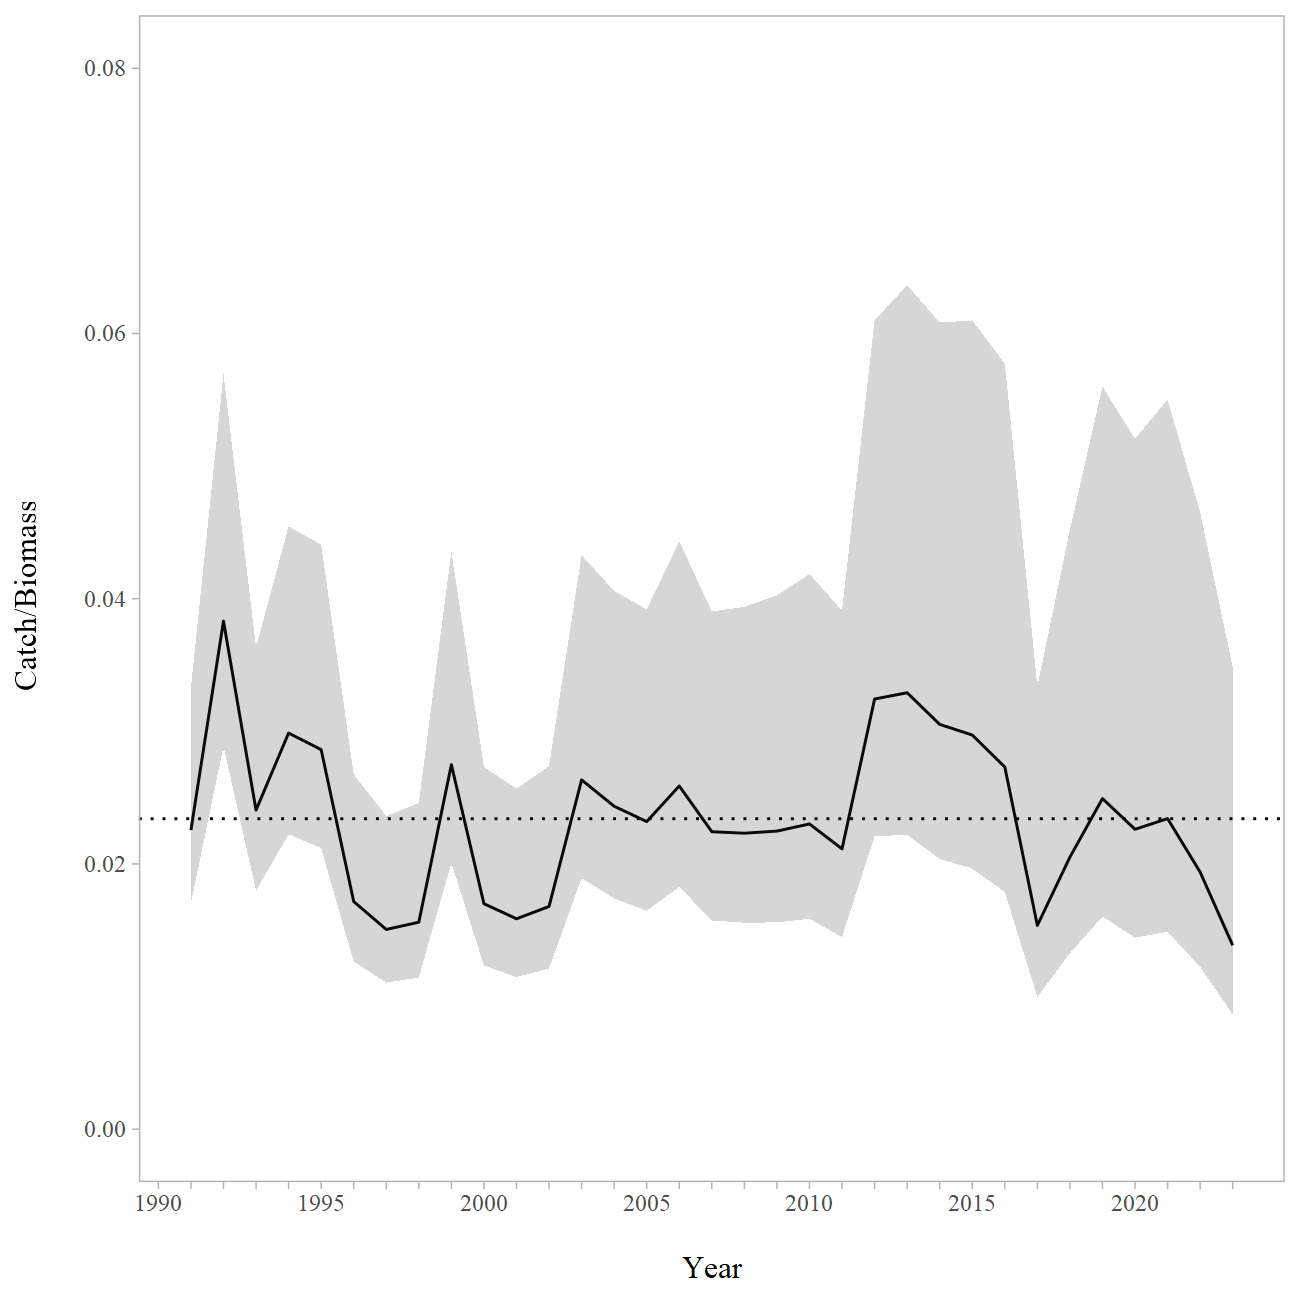
\includegraphics[width=18.06in,]{C:/Users/Ben.Williams/Work/assessments/northern_rockfish/2021/figs/catch_bio} \caption{Gulf of Alaska northern rockfish catch/age 2+ biomass ratio with approximate 95\% confidence intervals. Observed catch values were used for 1991-2020, the 2021 catch values were estimated using an expansion factor. The horizontal dashed line is the mean value for the entire dataset.}\label{fig:fig1}
\end{figure}

\begin{figure}[!h]
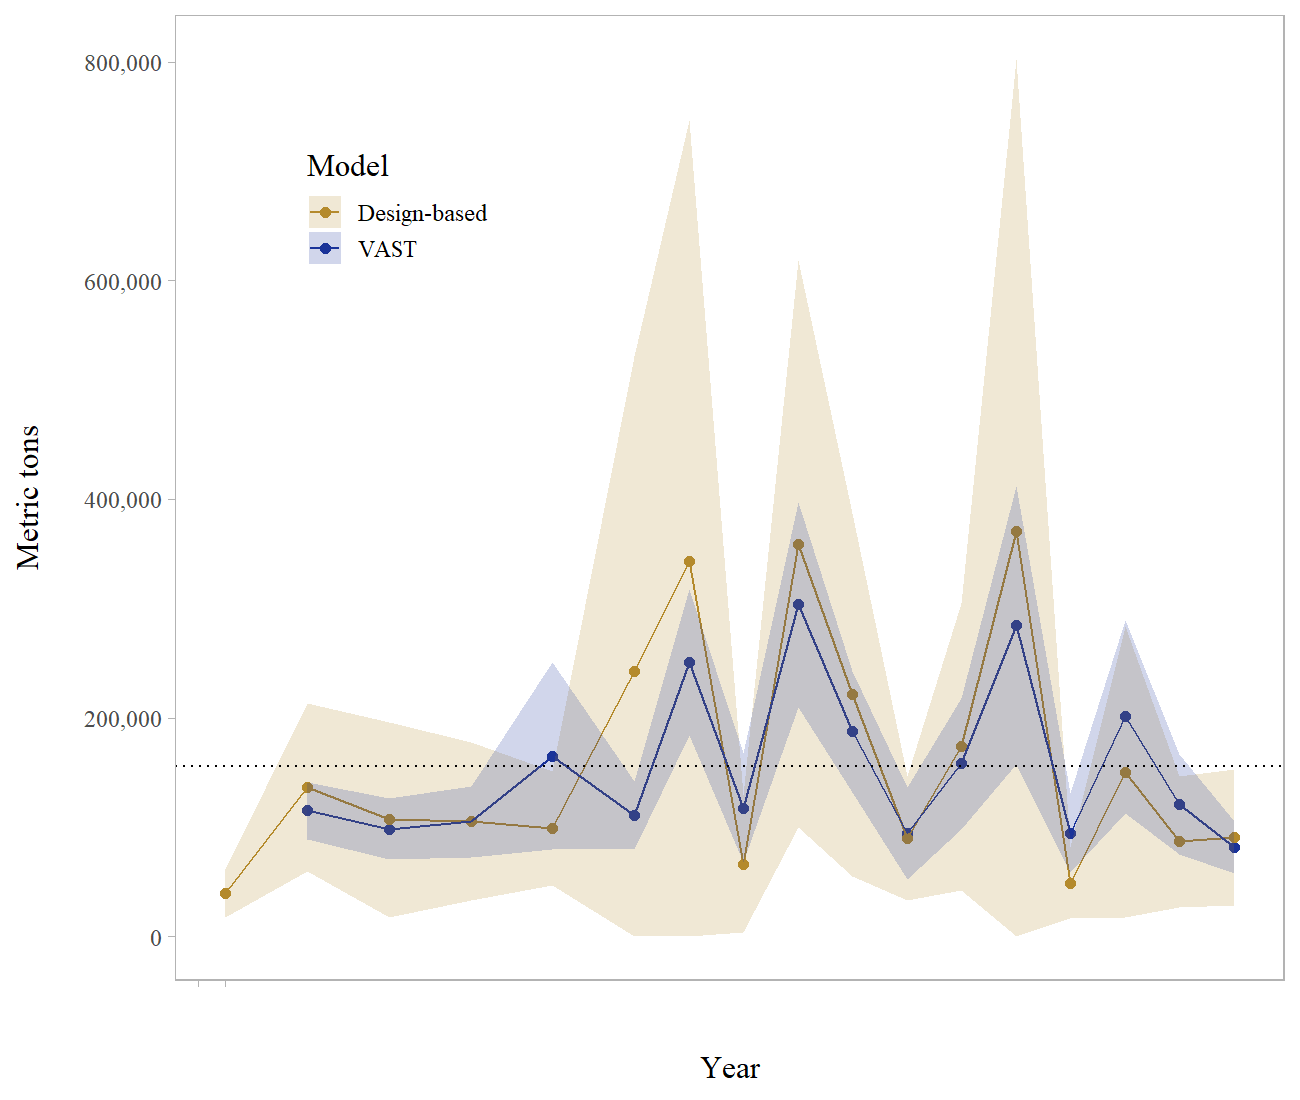
\includegraphics[width=18.06in,]{C:/Users/Ben.Williams/Work/assessments/northern_rockfish/2021/figs/ts_biomass} \caption{Geostatistical model (VAST) and design-based model estimates of trawl survey abundance for northern rockfish in the Gulf of Alaska. Shaded areas are 95\% confidence intervals, the dashed line is the data mean (VAST).}\label{fig:fig2}
\end{figure}

\pagebreak

\end{document}
